% Created by tikzDevice version 0.12.3.1 on 2022-05-01 19:45:56
% !TEX encoding = UTF-8 Unicode
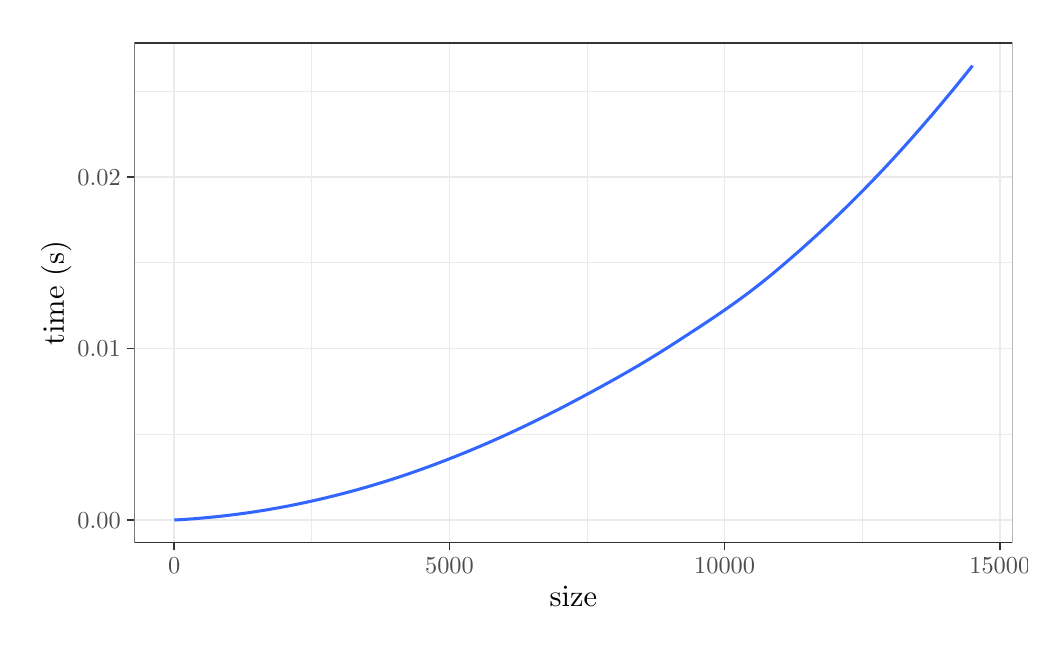
\begin{tikzpicture}[x=1pt,y=1pt]
\definecolor{fillColor}{RGB}{255,255,255}
\path[use as bounding box,fill=fillColor,fill opacity=0.00] (0,0) rectangle (361.35,216.81);
\begin{scope}
\path[clip] (  0.00,  0.00) rectangle (361.35,216.81);
\definecolor{drawColor}{RGB}{255,255,255}
\definecolor{fillColor}{RGB}{255,255,255}

\path[draw=drawColor,line width= 0.6pt,line join=round,line cap=round,fill=fillColor] (  0.00,  0.00) rectangle (361.35,216.81);
\end{scope}
\begin{scope}
\path[clip] ( 38.56, 30.69) rectangle (355.85,211.31);
\definecolor{fillColor}{RGB}{255,255,255}

\path[fill=fillColor] ( 38.56, 30.69) rectangle (355.85,211.31);
\definecolor{drawColor}{gray}{0.92}

\path[draw=drawColor,line width= 0.3pt,line join=round] ( 38.56, 69.83) --
	(355.85, 69.83);

\path[draw=drawColor,line width= 0.3pt,line join=round] ( 38.56,131.86) --
	(355.85,131.86);

\path[draw=drawColor,line width= 0.3pt,line join=round] ( 38.56,193.90) --
	(355.85,193.90);

\path[draw=drawColor,line width= 0.3pt,line join=round] (102.70, 30.69) --
	(102.70,211.31);

\path[draw=drawColor,line width= 0.3pt,line join=round] (202.13, 30.69) --
	(202.13,211.31);

\path[draw=drawColor,line width= 0.3pt,line join=round] (301.57, 30.69) --
	(301.57,211.31);

\path[draw=drawColor,line width= 0.6pt,line join=round] ( 38.56, 38.81) --
	(355.85, 38.81);

\path[draw=drawColor,line width= 0.6pt,line join=round] ( 38.56,100.84) --
	(355.85,100.84);

\path[draw=drawColor,line width= 0.6pt,line join=round] ( 38.56,162.88) --
	(355.85,162.88);

\path[draw=drawColor,line width= 0.6pt,line join=round] ( 52.98, 30.69) --
	( 52.98,211.31);

\path[draw=drawColor,line width= 0.6pt,line join=round] (152.42, 30.69) --
	(152.42,211.31);

\path[draw=drawColor,line width= 0.6pt,line join=round] (251.85, 30.69) --
	(251.85,211.31);

\path[draw=drawColor,line width= 0.6pt,line join=round] (351.29, 30.69) --
	(351.29,211.31);
\definecolor{drawColor}{RGB}{51,102,255}

\path[draw=drawColor,line width= 1.1pt,line join=round] ( 52.98, 38.90) --
	( 56.63, 39.11) --
	( 60.28, 39.38) --
	( 63.93, 39.69) --
	( 67.58, 40.04) --
	( 71.23, 40.44) --
	( 74.89, 40.88) --
	( 78.54, 41.37) --
	( 82.19, 41.90) --
	( 85.84, 42.48) --
	( 89.49, 43.11) --
	( 93.14, 43.78) --
	( 96.79, 44.50) --
	(100.44, 45.26) --
	(104.10, 46.07) --
	(107.75, 46.92) --
	(111.40, 47.82) --
	(115.05, 48.76) --
	(118.70, 49.74) --
	(122.35, 50.77) --
	(126.00, 51.85) --
	(129.65, 52.97) --
	(133.31, 54.14) --
	(136.96, 55.36) --
	(140.61, 56.63) --
	(144.26, 57.94) --
	(147.91, 59.29) --
	(151.56, 60.69) --
	(155.21, 62.13) --
	(158.86, 63.61) --
	(162.52, 65.13) --
	(166.17, 66.70) --
	(169.82, 68.31) --
	(173.47, 69.96) --
	(177.12, 71.66) --
	(180.77, 73.40) --
	(184.42, 75.18) --
	(188.07, 76.99) --
	(191.73, 78.85) --
	(195.38, 80.74) --
	(199.03, 82.67) --
	(202.68, 84.62) --
	(206.33, 86.60) --
	(209.98, 88.61) --
	(213.63, 90.65) --
	(217.28, 92.74) --
	(220.94, 94.87) --
	(224.59, 97.06) --
	(228.24, 99.30) --
	(231.89,101.61) --
	(235.54,103.97) --
	(239.19,106.34) --
	(242.84,108.72) --
	(246.49,111.14) --
	(250.15,113.61) --
	(253.80,116.15) --
	(257.45,118.76) --
	(261.10,121.47) --
	(264.75,124.29) --
	(268.40,127.23) --
	(272.05,130.30) --
	(275.70,133.43) --
	(279.36,136.63) --
	(283.01,139.89) --
	(286.66,143.24) --
	(290.31,146.65) --
	(293.96,150.15) --
	(297.61,153.72) --
	(301.26,157.38) --
	(304.91,161.12) --
	(308.57,164.95) --
	(312.22,168.87) --
	(315.87,172.87) --
	(319.52,176.95) --
	(323.17,181.11) --
	(326.82,185.35) --
	(330.47,189.67) --
	(334.12,194.07) --
	(337.78,198.55) --
	(341.43,203.10);
\definecolor{drawColor}{gray}{0.20}

\path[draw=drawColor,line width= 0.6pt,line join=round,line cap=round] ( 38.56, 30.69) rectangle (355.85,211.31);
\end{scope}
\begin{scope}
\path[clip] (  0.00,  0.00) rectangle (361.35,216.81);
\definecolor{drawColor}{gray}{0.30}

\node[text=drawColor,anchor=base east,inner sep=0pt, outer sep=0pt, scale=  0.88] at ( 33.61, 35.78) {0.00};

\node[text=drawColor,anchor=base east,inner sep=0pt, outer sep=0pt, scale=  0.88] at ( 33.61, 97.81) {0.01};

\node[text=drawColor,anchor=base east,inner sep=0pt, outer sep=0pt, scale=  0.88] at ( 33.61,159.85) {0.02};
\end{scope}
\begin{scope}
\path[clip] (  0.00,  0.00) rectangle (361.35,216.81);
\definecolor{drawColor}{gray}{0.20}

\path[draw=drawColor,line width= 0.6pt,line join=round] ( 35.81, 38.81) --
	( 38.56, 38.81);

\path[draw=drawColor,line width= 0.6pt,line join=round] ( 35.81,100.84) --
	( 38.56,100.84);

\path[draw=drawColor,line width= 0.6pt,line join=round] ( 35.81,162.88) --
	( 38.56,162.88);
\end{scope}
\begin{scope}
\path[clip] (  0.00,  0.00) rectangle (361.35,216.81);
\definecolor{drawColor}{gray}{0.20}

\path[draw=drawColor,line width= 0.6pt,line join=round] ( 52.98, 27.94) --
	( 52.98, 30.69);

\path[draw=drawColor,line width= 0.6pt,line join=round] (152.42, 27.94) --
	(152.42, 30.69);

\path[draw=drawColor,line width= 0.6pt,line join=round] (251.85, 27.94) --
	(251.85, 30.69);

\path[draw=drawColor,line width= 0.6pt,line join=round] (351.29, 27.94) --
	(351.29, 30.69);
\end{scope}
\begin{scope}
\path[clip] (  0.00,  0.00) rectangle (361.35,216.81);
\definecolor{drawColor}{gray}{0.30}

\node[text=drawColor,anchor=base,inner sep=0pt, outer sep=0pt, scale=  0.88] at ( 52.98, 19.68) {0};

\node[text=drawColor,anchor=base,inner sep=0pt, outer sep=0pt, scale=  0.88] at (152.42, 19.68) {5000};

\node[text=drawColor,anchor=base,inner sep=0pt, outer sep=0pt, scale=  0.88] at (251.85, 19.68) {10000};

\node[text=drawColor,anchor=base,inner sep=0pt, outer sep=0pt, scale=  0.88] at (351.29, 19.68) {15000};
\end{scope}
\begin{scope}
\path[clip] (  0.00,  0.00) rectangle (361.35,216.81);
\definecolor{drawColor}{RGB}{0,0,0}

\node[text=drawColor,anchor=base,inner sep=0pt, outer sep=0pt, scale=  1.10] at (197.20,  7.64) {size};
\end{scope}
\begin{scope}
\path[clip] (  0.00,  0.00) rectangle (361.35,216.81);
\definecolor{drawColor}{RGB}{0,0,0}

\node[text=drawColor,rotate= 90.00,anchor=base,inner sep=0pt, outer sep=0pt, scale=  1.10] at ( 13.08,121.00) {time (s)};
\end{scope}
\end{tikzpicture}
